\documentclass{aps2010} \special{papersize=8.5in,11in}
%\usepackage{hyperref}
%\usepackage{sectsty}
%\sectionfont{\fontfamily{ptm}\selectfont}

\usepackage{times}
\usepackage{rawfonts}
\usepackage{graphicx}

\title{Element gain drifts as an imaging dynamic range limitation\\in PAF-based
interferometers}

%% the organization option [orgN] associates the authors with his
%% proper address
\author[org1]{\textbf{\underline{\emph{O.M. Smirnov}}}}
\author[org2]{\textbf{\emph{M.V. Ivashina}}}

%% each address must have a unique identifier in the option field
\address[org1]{ASTRON, P.O. Box 2, Dwingeloo, 7900AA, The Netherlands, smirnov@astron.nl}
\address[org2]{Dept. of Earth and Space Sciences, Chalmers University of Technology, S-41296 Gothenburg, Sweden, marianna.ivashina@chalmers.se}

\begin{document}

\maketitleblock

\begin{abstract}
These instructions explain the process for preparing and submitting
the program abstract and paper for the URSI General Assembly and
Scientific Symposium (GASS). Both the program abstract and the paper
are to be submitted online, using the Web site at
http://www.papers-gass2011.ursi.org/welcome.asp. The program
abstract (which is separate from and independent of the abstract for
the paper) is to consist of no more than 100 words, and is entered
online using only plain text. It will appear in the hardcopy
Abstracts Book, and be used by attendees to help choose which papers
to attend. The paper is to be prepared and submitted as a PDF file.
It will be reviewed as part of the acceptance process for GASS
papers, and if accepted it will appear in the CD-ROM
\emph{Proceedings} of the GASS. If the paper is presented at the
GASS, it will appear in IEEE Xplore.
\end{abstract}

\section*{Introduction}


\section{Beamforming and compound beams}

An EMF propagating as a transverse plane wave, arriving from any given direction on the sky $\vec\sigma$, can be 
instantaneously characterized by two complex amplitudes $\epsilon_x,\epsilon_y$. The nominal ``voltage'' response $v$ of a single   
compound beam (composed from $n$ PAF elements) for the given direction can then be described by a chain of matrix products:

\begin{equation}
v =
\left( 
  \begin{array}{ccc}
  w_{1} & \ldots w_n 
  \end{array} 
\right)
\left( 
  \begin{array}{ccc}
  g_{1} & & 0\\
  & \ddots & \\
  0 & & g_n  
  \end{array} 
\right) 
\left( 
  \begin{array}{cc}
  e_{x1} & e_{y1} \\
  \vdots & \vdots \\
  e_{xn} & e_{yn} 
  \end{array} 
\right) 
\left(
  \begin{array}{c}
  \epsilon_x \\
  \epsilon_y
  \end{array} 
\right), \\
\end{equation}

i.e. simply as $v=\vec w^T \mathbf{G} \mathbf{E} \vec\epsilon$, where $\mathbf{E}$ is a $n\times2$ matrix of direction-dependent beam gains associated with each element, $\mathbf{G}$ is a diagonal matrix of LNA gains (one per element), and $\vec w$ is a vector of beamformer weights. The row 2-vector given by $\vec w^T \mathbf{G} \mathbf{E}$ can be thought of as the compound beam gain. To measure polarization, we form a pair of compound beams (using different sets of weights) that are preferentially sensitive to the $x$ or $y$ component of the EMF. The two row vectors $\vec w_x^T \mathbf{G} \mathbf{E}$ and $\vec w_y^T \mathbf{G} \mathbf{E}$ then form the rows of the ``E-Jones'' matrix corresponding to this pair of beams (Fig.~\ref{fig:jones-matrix}). This is done for every ``look direction'' into which we want to point a compound beam, so in total we have 74 compound beams, of which half are polarized in $x$, and half in $y$.

In an interferometer, the signals from each pair of beams are correlated between every station of the interferometer array, forming up a total of four correlations per baseline ($xx$, $yy$, $xy$ and $yx$), per 37 synthesized pointings. The resulting complex visibilities can be described using a Jones or Mueller formalism of the radio interferometry measurement equation (RIME) [2-3].

By choosing different weighting vectors $\vec w_x,\vec w_y$, we 6can choose to optimize different aspects of the resulting compound beams, such as sensitivity, SNR, shape, instrumental polarization, etc. This is an art unto itself\footnote{NB: Marianna, if there's a separate section about this in Oleg's paper, then this text needs to be modified. For URSI, we'll just cite your paper, and any other relevant ones.}. For the purposes of this study, we concern ourselves with a different question: how does the behaviour of $\mathbf{G}$ influence our compound beam, and how (or if) this in turn affects our ability to reconstruct images from the measured visibilities.

\section{Element gain drifts}

The LNA gains given by $\mathbf{G}$ are in principle unknown, and drift in time (independently of each other) in response to changing environmental conditions. During initial beamformer calibration\footnote{NB: Marianna, this needs to be described in your terminology. Do you even call it ``beamformer calibration'', or something else?}, the current element gains are estimated, and a suitable weight vector is chosen to compensate (so that the product $\vec w^T\mathbf{G}$ is equivalent to a set of ``ideal'' weights that would be used if the gains were unity). From that point, $\mathbf{G}$ begins drifting, resulting in a compound beam that slowly distorts in an unpredictable way (see Fig.~\ref{fig:gains}). 

Classic interferometry (and the self-calibration algorithm in particular) implicitly assumes that all stations of an interferometer array have an identical and stable beam response. Element gain drifts (EGDs) break this assumption, resulting in a time-variable, station-dependent, direction-dependent effect (DDE). This in turn produces subtle (or not so subtle) artefacts in interferometric images; see [5] for a more detailed look at this error mechanism. If these artefacts are sufficiently high (compared to the thermal noise), they could effectively limit the dynamic range
(DR) of the resulting images. Conversely, our imaging DR requirements effectively determine how much EGD we can tolerate in the system, and can thus be translated into beamformer calibration and/or hardware requirements.

It is, however, very difficult to relate EGDs to the level of interferometric artefacts analytically. We have therefore decided to conduct a series of numerical simulations using the MeqTrees package [6]. The resulting simulations framework and methodology
can be readily applied to other PAF designs, and even to aperture arrays.

\section{Simulations}

The inputs to our simulator are a set of element beam patterns (specified as FITS files), one per each element, a set of weight vectors $\vec w_{ij}$ (per each polarization direction $i=x,y$ and pointing $j=1\ldots37$) corresponding to the desired compound beams\footnote{NB: Marianna, some words here on where the weights come from.}. This is combined with a {\em sky model} (a list of sources, essentially). For a given pointing, the simulator then works out the per-station compound beam gain in the direction of every source in the model, and evaluates a RIME that gives the resulting visibilities, which are written to a CASA-format Measurement Set (MS), which can then be imaged using standard tools (CASA or lwimager). Observational parameters, array layout, etc., are determined by the metadata of the MS. For our initial study, we simulated a 12-hour synthesis using the WSRT (with hypothetical Apertif front-ends) at 1.4 GHz. 

Since we wanted to have a clear indication of how the relative effect varied as a function of direction, we used a ``gridded sky'' model of $11\times11$ identical unpolarized 1~Jy point sources, arranged in a grid with a step of $12'$ (thus going out to $1^\circ$ from center in both directions). Simulating ``real'' observations with Apertif is just a matter of feeding the simulator a realistic sky model; for our purposes the gridded sky was actually preferable.

For the first (``reference'') simulation, we applied the nominal beam weights with no drift ($\mathbf{G}\equiv1$). The resulting $IQUV$ images are still quite informative, since they clearly show the distribution of instrumental polarization (due to different $x$ and $y$ beams, and cross-terms in the Jones matrix) over a single compound beam. Since the model sources have only $I$ flux, everything that makes its way into the $QUV$ maps is a result of instrumental polarization. Figure~\ref{fig:quv} shows the $QUV$ maps for pointing 16, which is well off the optical axis of the dish. The most striking feature is the complicated behaviour as a function of direction. (Note that the images in effect show a combination of three things: instrumental polarization per se, attenuated by the overall power beam, and convolved with the point spread function of the interferometer.) 

We then allowed $\mathbf{G}$ to drift as a function of time. For this initial study, we used a very primitive EGD model: the complex amplitude and phase of every element of $\mathbf{G}$ was modulated by a  sine wave, with a randomly-chosen period (between 2 and 6 hours) and initial phase. The amplitude was modulated by $\pm0.5$ dBA, and the phase by $\pm10$ degrees\footnote{NB: Marianna, maybe some words about where we got these figures, and how we'll put in more realistic ones in the future?}. Each station's $\mathbf{G}$ was subject to its own modulation. A summary plot of the resulting compound beam gains (as a function of time) for a few directions and stations can be seen in Fig.~\ref{fig:gains}. We call this the ``error'' simulation.

\section{Errors and dynamic range}

The resulting ``error'' images cannot be distinguished from the ``reference'' images by eye alone, since the effect is quite subtle. The difference between the two sets of images, however, is quite striking (Fig.~\ref{fig:diff-uncal}). This indicates both the distribution of the artefacts, and their level, which corresponds to a DR limit of about 100.

Such DR is pathetic by radio interferometric standards. Fortunately, self-calibration can correct for some of it. Given a dominant source, selfcal can estimate the overall gain \underline{in the direction of that source}, and correct for it. Any remaining artefacts are then due to the gain \emph{differences} between the dominant source and the other sources in the field, and increase (in relative level) as one gets further away from the dominant source. (These are often called off-axis artefacts, since conventional interferometric practice puts the dominant source in the centre of the beam, i.e. ``on-axis''. For Apertif this is no longer the case, so the term DDEs is preferred.) 

We can simulate the effect of a ``perfect'' selfcal (for e.g. a dominant source at the centre) by dividing the beam gain in each direction by the beam gain towards the central source. This results in a set of ``corrected'' images. By imaging the difference between these and the ``reference'' images (Fig.~\ref{fig:diff-cal}), we get a clear indication of the artefact level after selfcal. Note how the artefacts go from none at centre (since that's the direction towards which the gain has been corrected), to a maximum somewhere around the half-power point, and then back to zero (as the primary beam power tails off). Note also that there's little difference in the error level between the on-axis and off-axis compound beams, it is only the distribution of the artefacts that differs. The corresponding DR limitation after classic selfcal is on the order of 1000.

This may still seem low, but recall that the dominant source would be taken care of by selfcal, so it is only the remaining sources that would leave artefacts on a \emph{relative} level of $10^{-3}$. If these sources are relatively faint, the \emph{absolute} artefact level may be tolerably low. In fact, current single-pixel-feed WSRT observations at 1.4 GHz exhibit about the same relative artefact level on off-axis sources (assuming a dominant source on-axis, which is corrected for by selfcal), which is thought to be due to pointing errors and other mechanical effects [7].

We can therefore conclude that the DR limitations due to our simulated EGDs are on roughly the same order as the ``hard'' limits imposed by the 
WSRT's existing optics and mechanics. In other words, they will not constitute a DR limitation, and will be drowned out by other effects, if only real-life EGDs prove to be somewhat lower than those we have put into the simulation. It is the latter clause that requires additional work. We are currently awaiting the results of a measurement campaign on the current Digestif prototype, which should give us a handle on real-life EGDs, and allow us to come to a  definitive answer on the DR issue.

\section{Conclusions and future work}

The tools and methodology presented here provides the missing link between the electromagnetic simulations of antenna engineers, and the 
imaging requirements of astronomers. It is flexible enough that we can simulate wildly different PAF and AA configurations, and determine how these ultimately influence dynamic range.

In the particular case of Apertif, if real-life EGDs prove to be somewhat lower than those used for our initial simulations, the dynamic range of Apertif will be limited by WSRT hardware, and not the EGDs per se. Further work is required to establish this conclusively.

\begin{figure}
Marianna needs to prepare this figure, and check the caption.
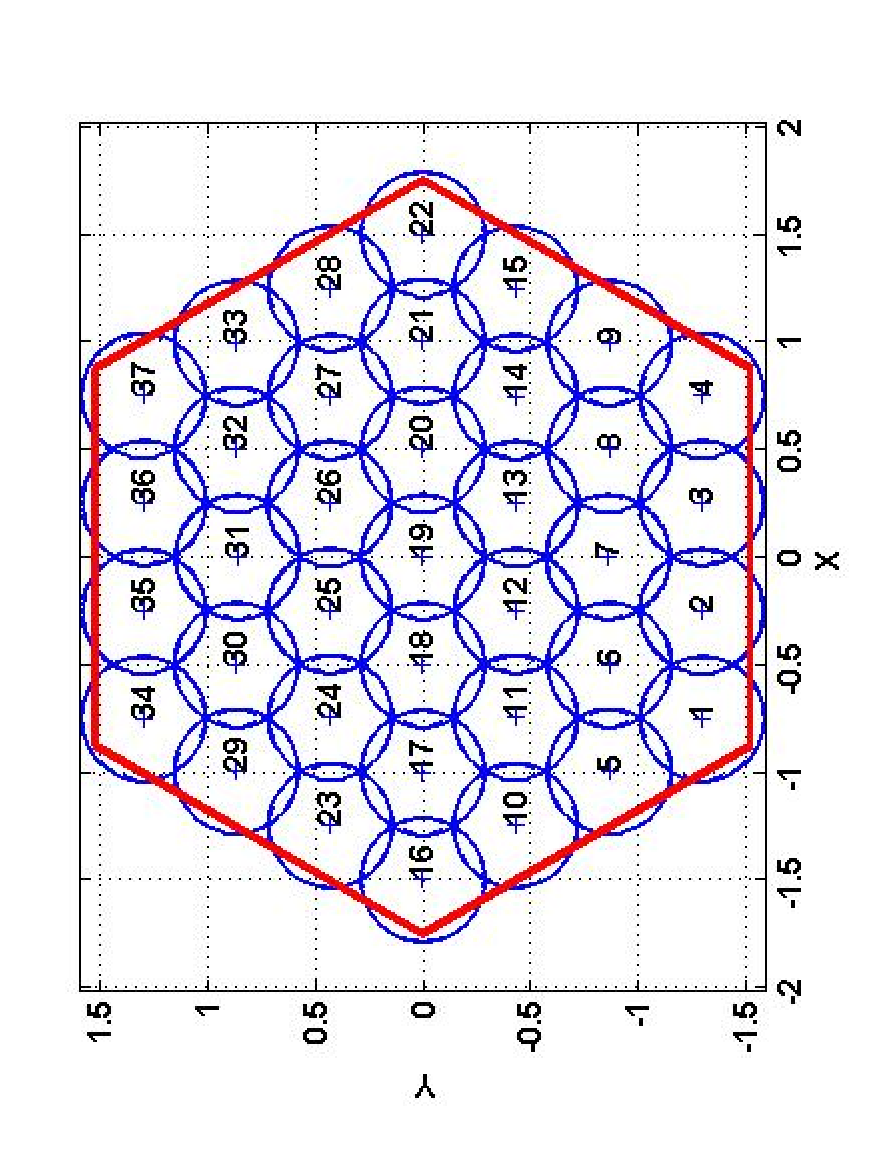
\includegraphics[width=9cm]{ArrangementOfBeams} 
\caption{\label{fig:apertif}Digestif prototype (left) and the distribution of compound beams over the full field-of-view (right).}
\end{figure}


\begin{figure}
Marianna needs to prepare this figure. 
\caption{\label{fig:jones-matrix}Jones matrices for the beam gain of compound beams 19 (left) and 16 (right).
Beam 19 points along the optical axis, beams 16 is the furthest off-axis, pointing XXXX due West. The four plots (per beam) 
show the complex amplitude of $j_{11},j_{12}$ (top row) and $j_{21},j_{22}$ (bottow row) as a function of direction.
}
\end{figure}


\begin{figure}
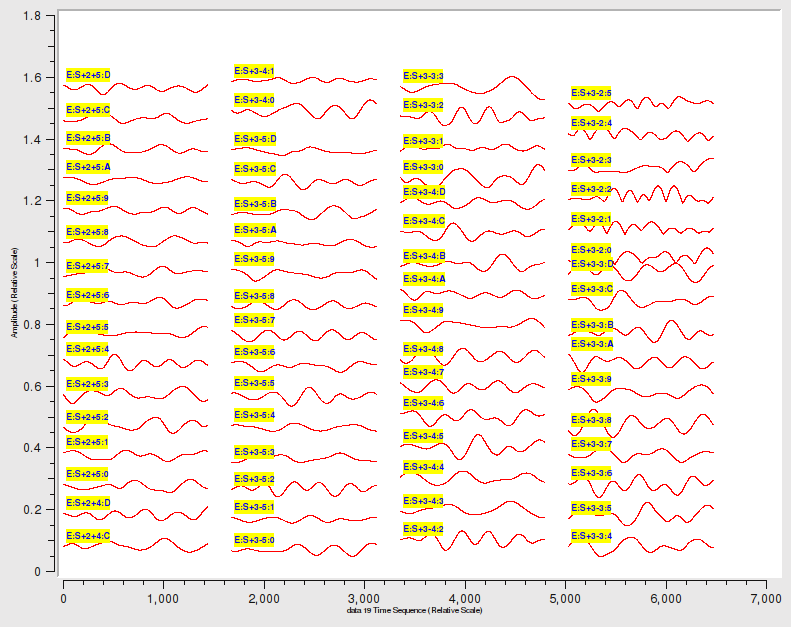
\includegraphics[width=9cm]{inspector_gains1}%
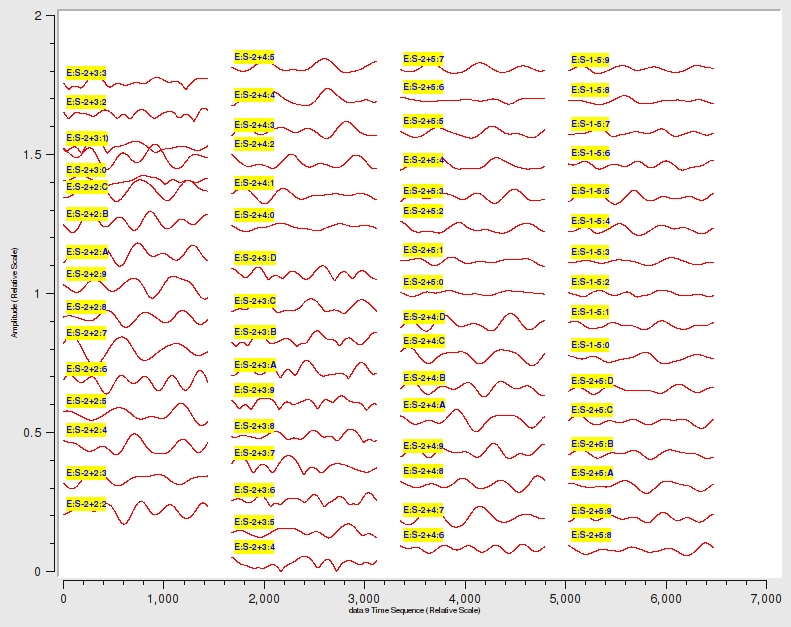
\includegraphics[width=9cm]{inspector_gains2} 
\caption{\label{fig:gains}An example of the compound beam gains produced during the simulation. Each track shows the gain-amplitude in the direction of one source, per one WSRT station, as a function of time.}
\end{figure}

\begin{figure}
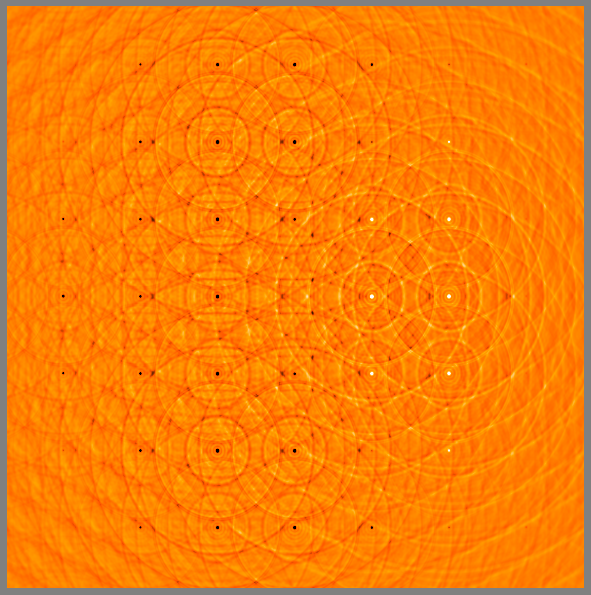
\includegraphics[width=6cm]{q15}%
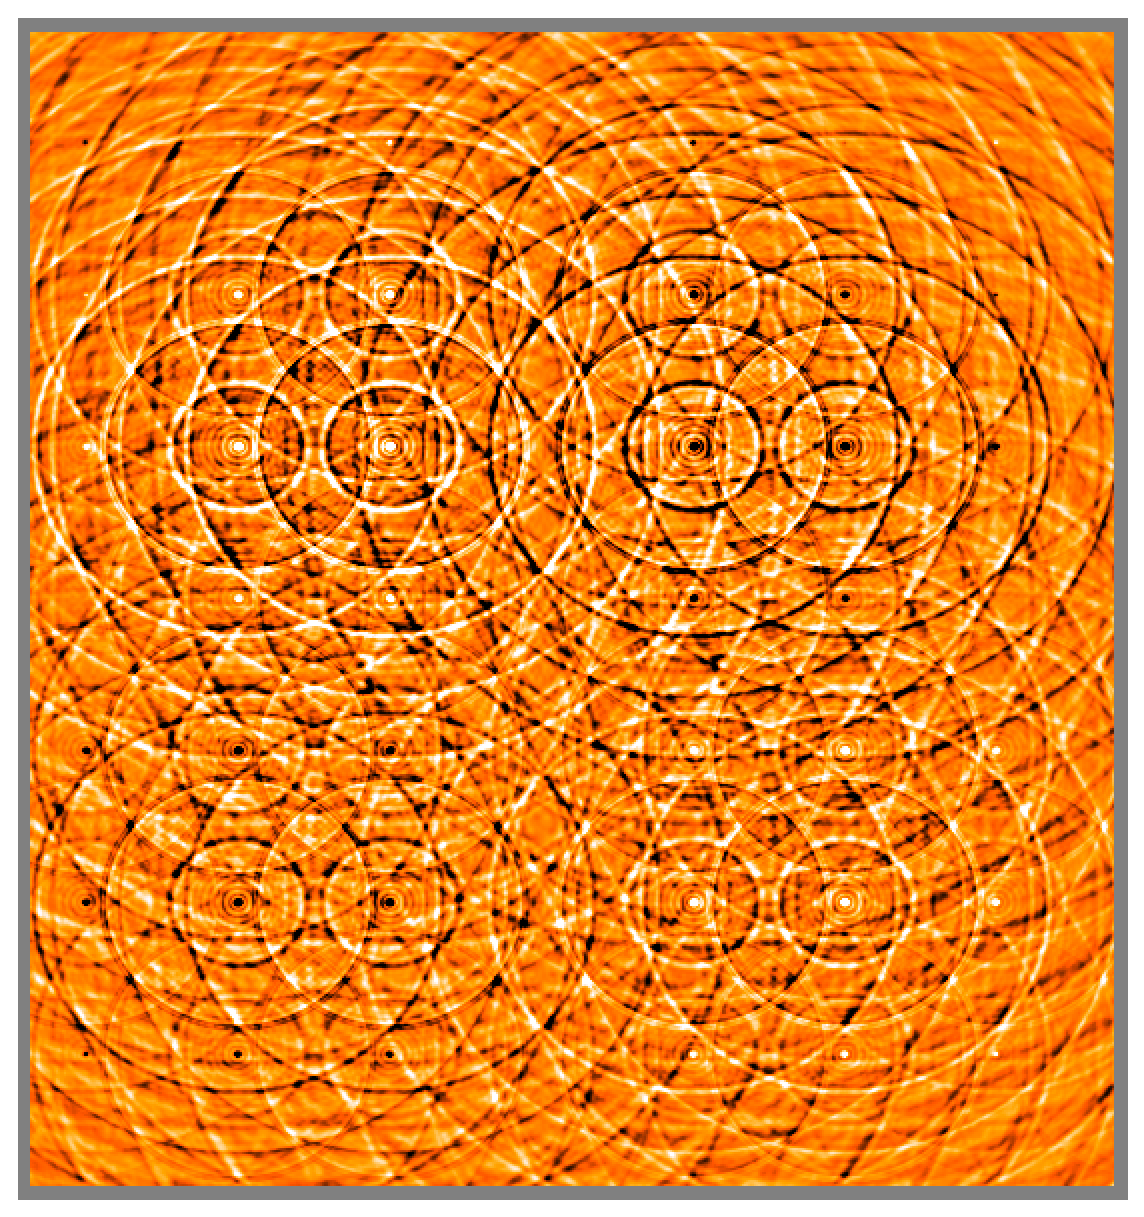
\includegraphics[width=6cm]{u15}%
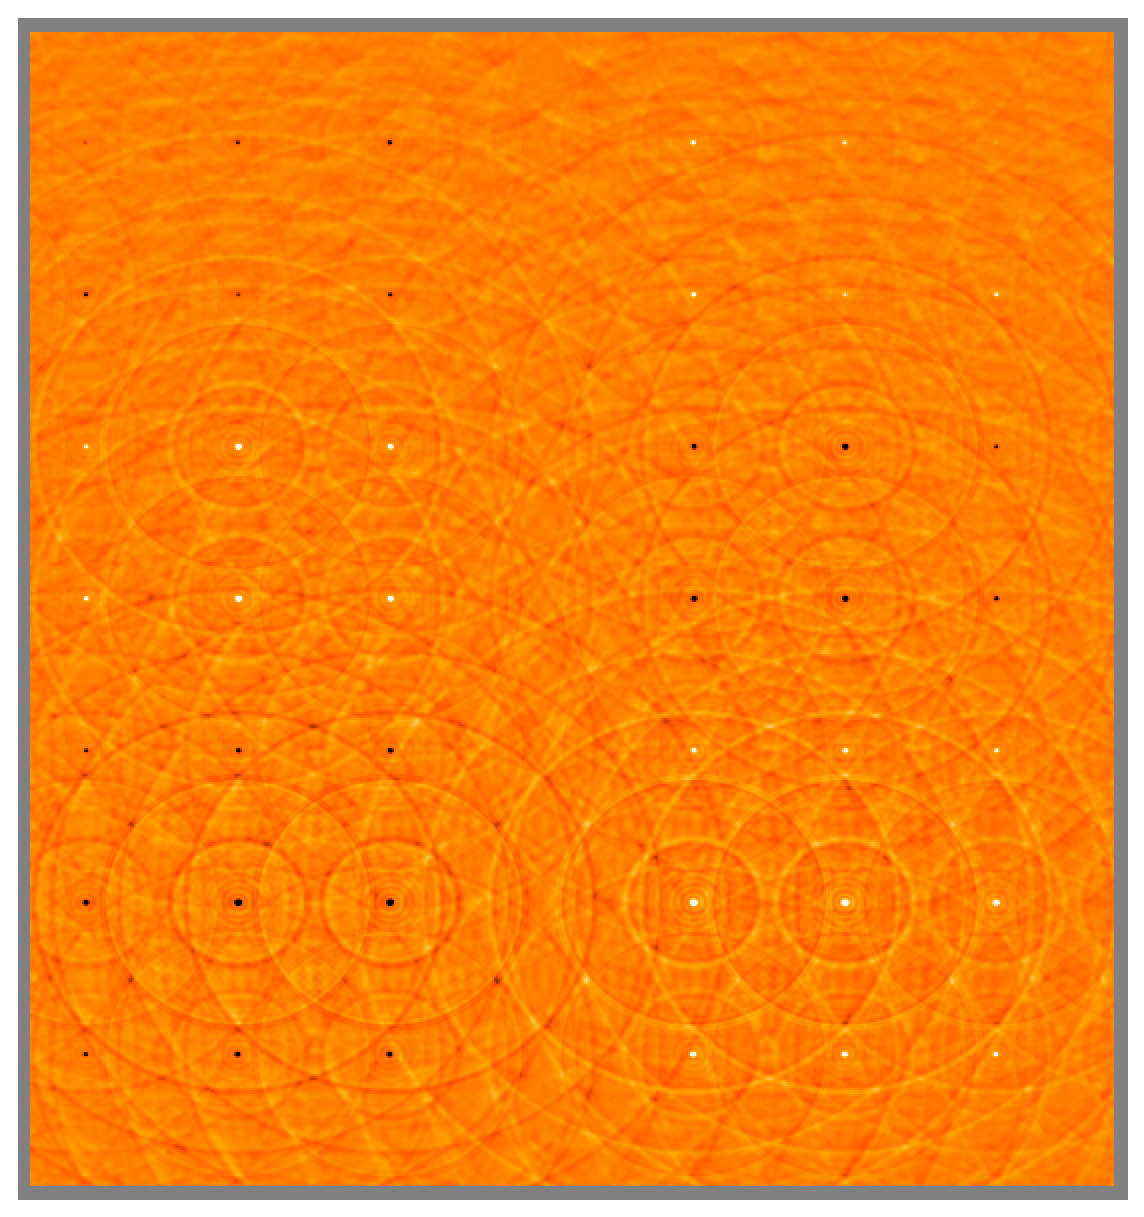
\includegraphics[width=6cm]{v15}
\caption{\label{fig:quv}$Q$, $U$, and $V$ maps showing a simulation without EGDs for beam 16. Model sources are 1 Jy unpolarized, so all this is purely instrumental polarization. The images are $\sim1.5^\circ$ across. The intensity range shown is $\pm2$~mJy (actual extremes are on the order of 20~mJy). Note the relatively high $U$, and the asymmetry in all three images. This is characteristic of Apertif's off-axis beams.}
\end{figure}

\begin{figure}
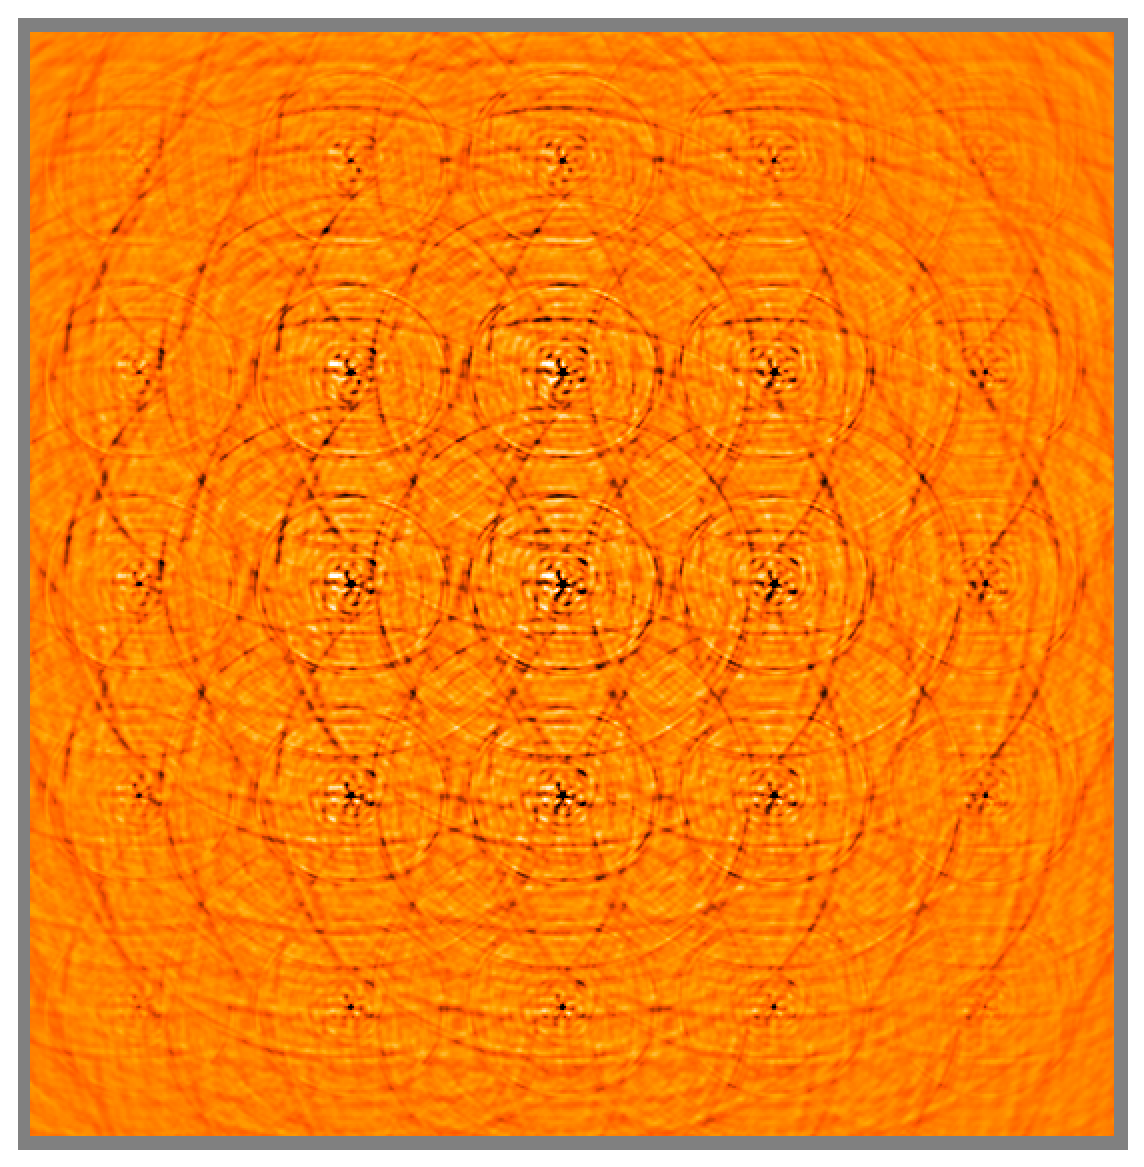
\includegraphics[width=9cm]{diff15uncal}%
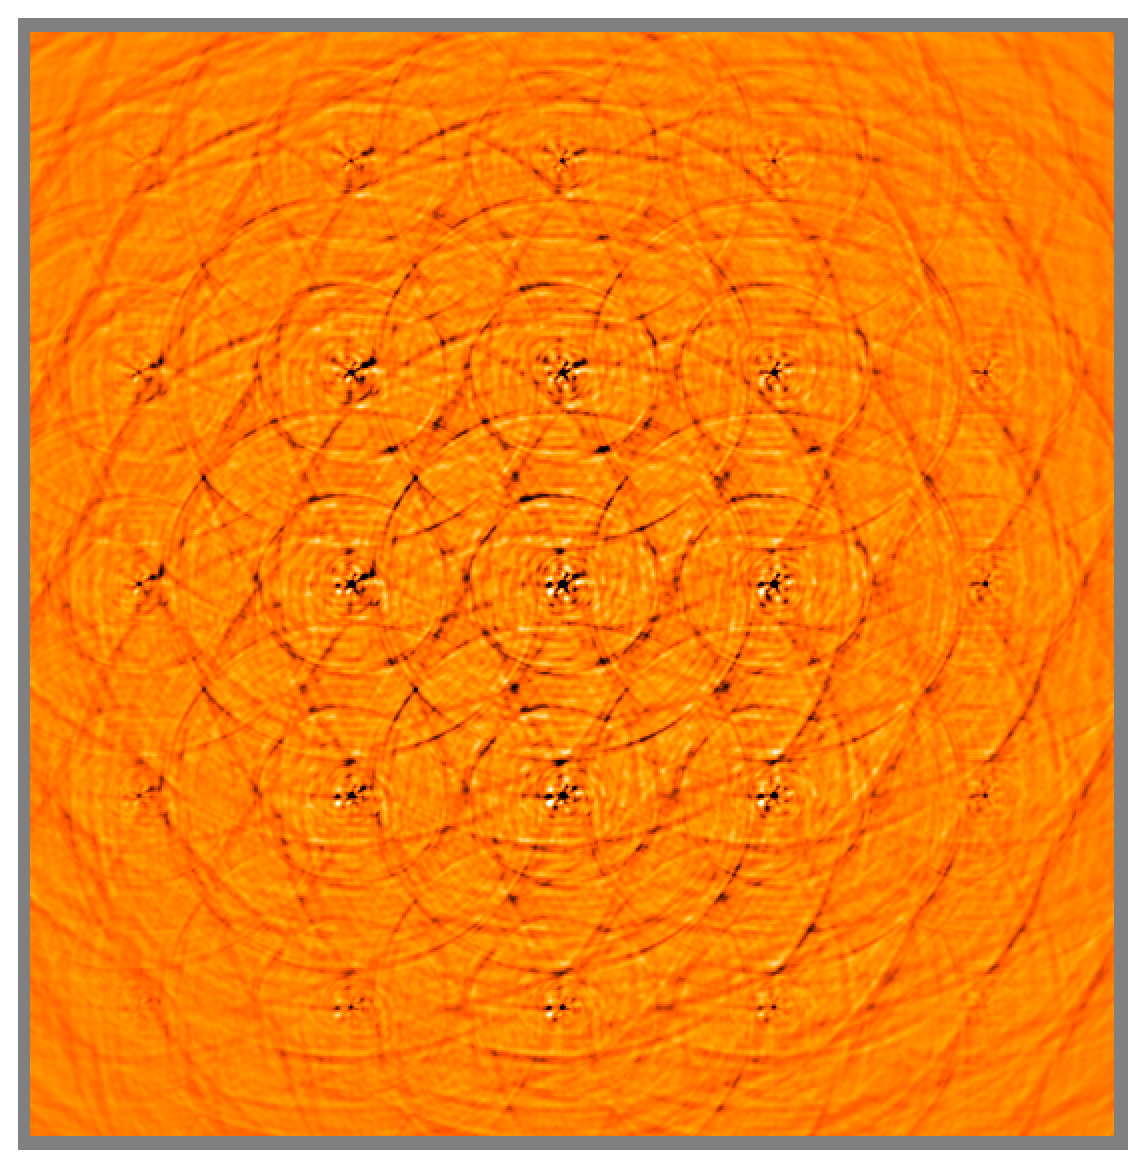
\includegraphics[width=9cm]{diff18uncal}%
\caption{\label{fig:diff-uncal}Imaging artefacts in Stokes $I$ due to EGDs. This shows the difference between the ``error'' and the ``reference'' images (see text) for beam 16 (left) and 19 (right). The images are $\sim1^\circ$ across. The intensity range shown is $\pm3$~mJy (actual extremes are on the order of 10~mJy).}
\end{figure}

\begin{figure}
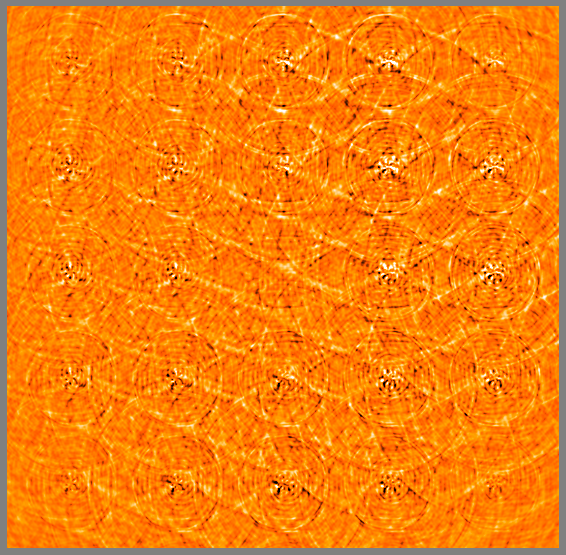
\includegraphics[width=9cm]{diff15cal}%
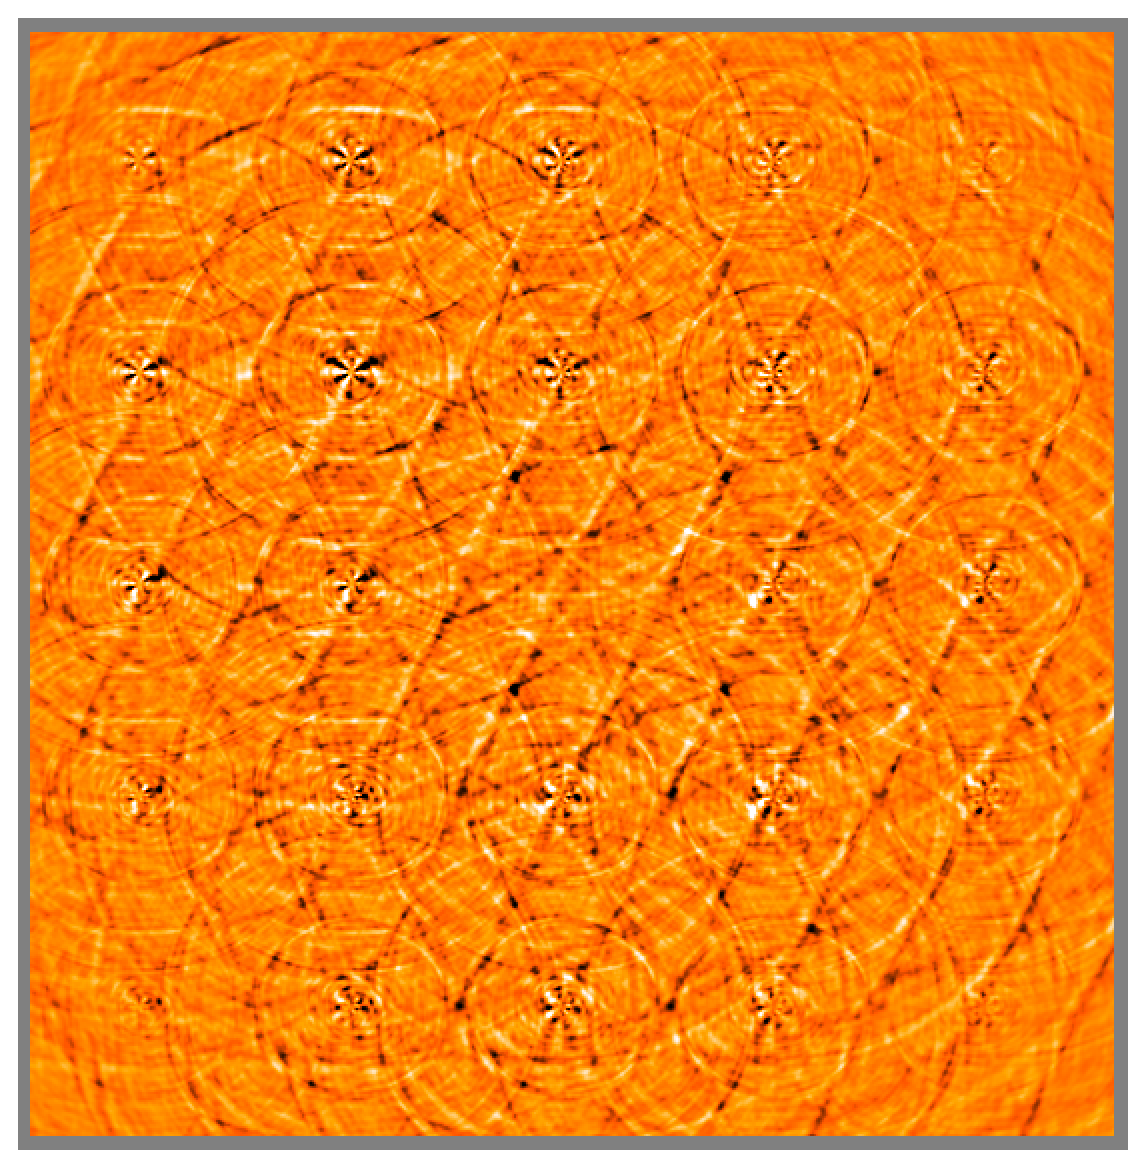
\includegraphics[width=9cm]{diff18cal}%
\caption{\label{fig:diff-cal}Imaging artefacts in Stokes $I$ after selfcal for beam 16 (left) and 19 (right). Note how the central source is corrected for. The images are $\sim1^\circ$ across. The intensity range shown is $\pm1$~mJy (actual extremes are on the order of 2~mJy).}
\end{figure}

\section{References}

\noindent 1. W. A. van Capellen and L. Bakker, ``APERTIF: Phased array feeds for the Westerbork Synthesis Radio Telescope'', \emph{Proceedings of the IEEE International Symposium on Phased Array Systems and Technology (ARRAY 2010)}, Waltham, MA, 2010, pp. 640--647

\noindent 2. J. P. Hamaker, J. D. Bregman and R. J. Sault, ``Understanding radio polarimetry. I. Mathematical foundations'', 
\emph{Astronomy \& Astrophysics Supp. Ser.}, 117, May 1996, pp. 137--147

\noindent 3. J. P. Hamaker, ``Understanding radio polarimetry. IV. The full-coherency analogue of scalar self-calibration: Self-alignment, dynamic range and polarimetric fidelity''.
\emph{Astronomy \& Astrophysics Supp. Ser.}, 143, May 2000, pp. 515--534

\noindent 4. O. A. Iupikov, M. V. Ivashina and O.M. Smirnov, ``Reducing the complexity of the beam calibration models of phased-array radio telescopes'', \emph{Proceedings of the 5th European Conference on Antennas and Propagation (EuCAP 2011)}, Rome, Italy, 2011

\noindent 5. O. M. Smirnov, ``Revisiting the radio interferometer measurement equation. II. Calibration and direction-dependent effects'',
\emph{Astronomy \& Astrophysics}, 527, March 2011, p. A107

\noindent 6. J. E. Noordam and O. M. Smirnov, ``The MeqTrees software system and its use for third-generation calibration of radio interferometers'',
\emph{Astronomy \& Astrophysics}, 524, December 2010, p. A61

\noindent 7. O. M. Smirnov, ``Revisiting the radio interferometer measurement equation. III. Addressing direction-dependent effects in 21cm WSRT observations of 3C 147'',
\emph{Astronomy \& Astrophysics}, 527, March 2011, p. A108


\end{document}
